\chapter{Theory and Background} \label{ch:background}
This chapter provides the theoretical foundation for the thesis, focusing strictly on the mechanics of sequential modeling and the time-shift anomaly. Section~\ref{sec:bg:models} introduces the deep learning architectures. Section~\ref{sec:bg:losses} details the mathematical formulations of the evaluated loss functions. Section~\ref{sec:bg:metrics} defines the point-wise and event-centric evaluation metrics, and Section~\ref{sec:bg:relwork} discusses related work in glucose forecasting.

% ================================================================
\section{Deep Learning for Time Series Forecasting} \label{sec:bg:models}
% ================================================================
\subsection{Long Short-Term Memory Networks} \label{sec:bg:models:lstm}
\begin{planned}
    \item Theoretical foundation of recurrent neural networks for sequential data and the resolution of the vanishing gradient problem.
    \item Mathematical mechanics of the input, forget, and output gating mechanisms.
    \item Brief specification of the chosen baseline recurrent network topology (two stacked layers, hidden size 256).
    \item \textit{Note: The full architecture diagram is provided in Appendix~\ref{appendix:architectures}.}
\end{planned}

\subsection{PatchTST} \label{sec:bg:models:patchtst}
\begin{planned}
    \item Review of self-attention mechanisms and the core design of the PatchTST architecture (segmentation into overlapping patches).
    \item Mathematical framework of Reversible Instance Normalization (RevIN) utilized to stabilize training.
    \item Analysis of the structural consequence of instance normalization, which strips absolute level info and compromises classification against static boundaries.
    \item \textit{Note: The full architecture diagram is shown in Fig.~\ref{fig:app:patchtst_arch} (Appendix~\ref{appendix:architectures}).}
\end{planned}

% ================================================================
\section{Loss Functions for Sequential Regression} \label{sec:bg:losses}
% ================================================================

\subsection{Mean Squared Error} \label{sec:bg:losses:mse}
\begin{planned}
    \item Definition of MSE as the average squared difference between each predicted and true value.
    \item Key limitation: MSE penalises a prediction that is correct in shape but slightly shifted in time just as harshly as a completely wrong prediction.
\end{planned}

\begin{figure}[htbp]
    \centering
    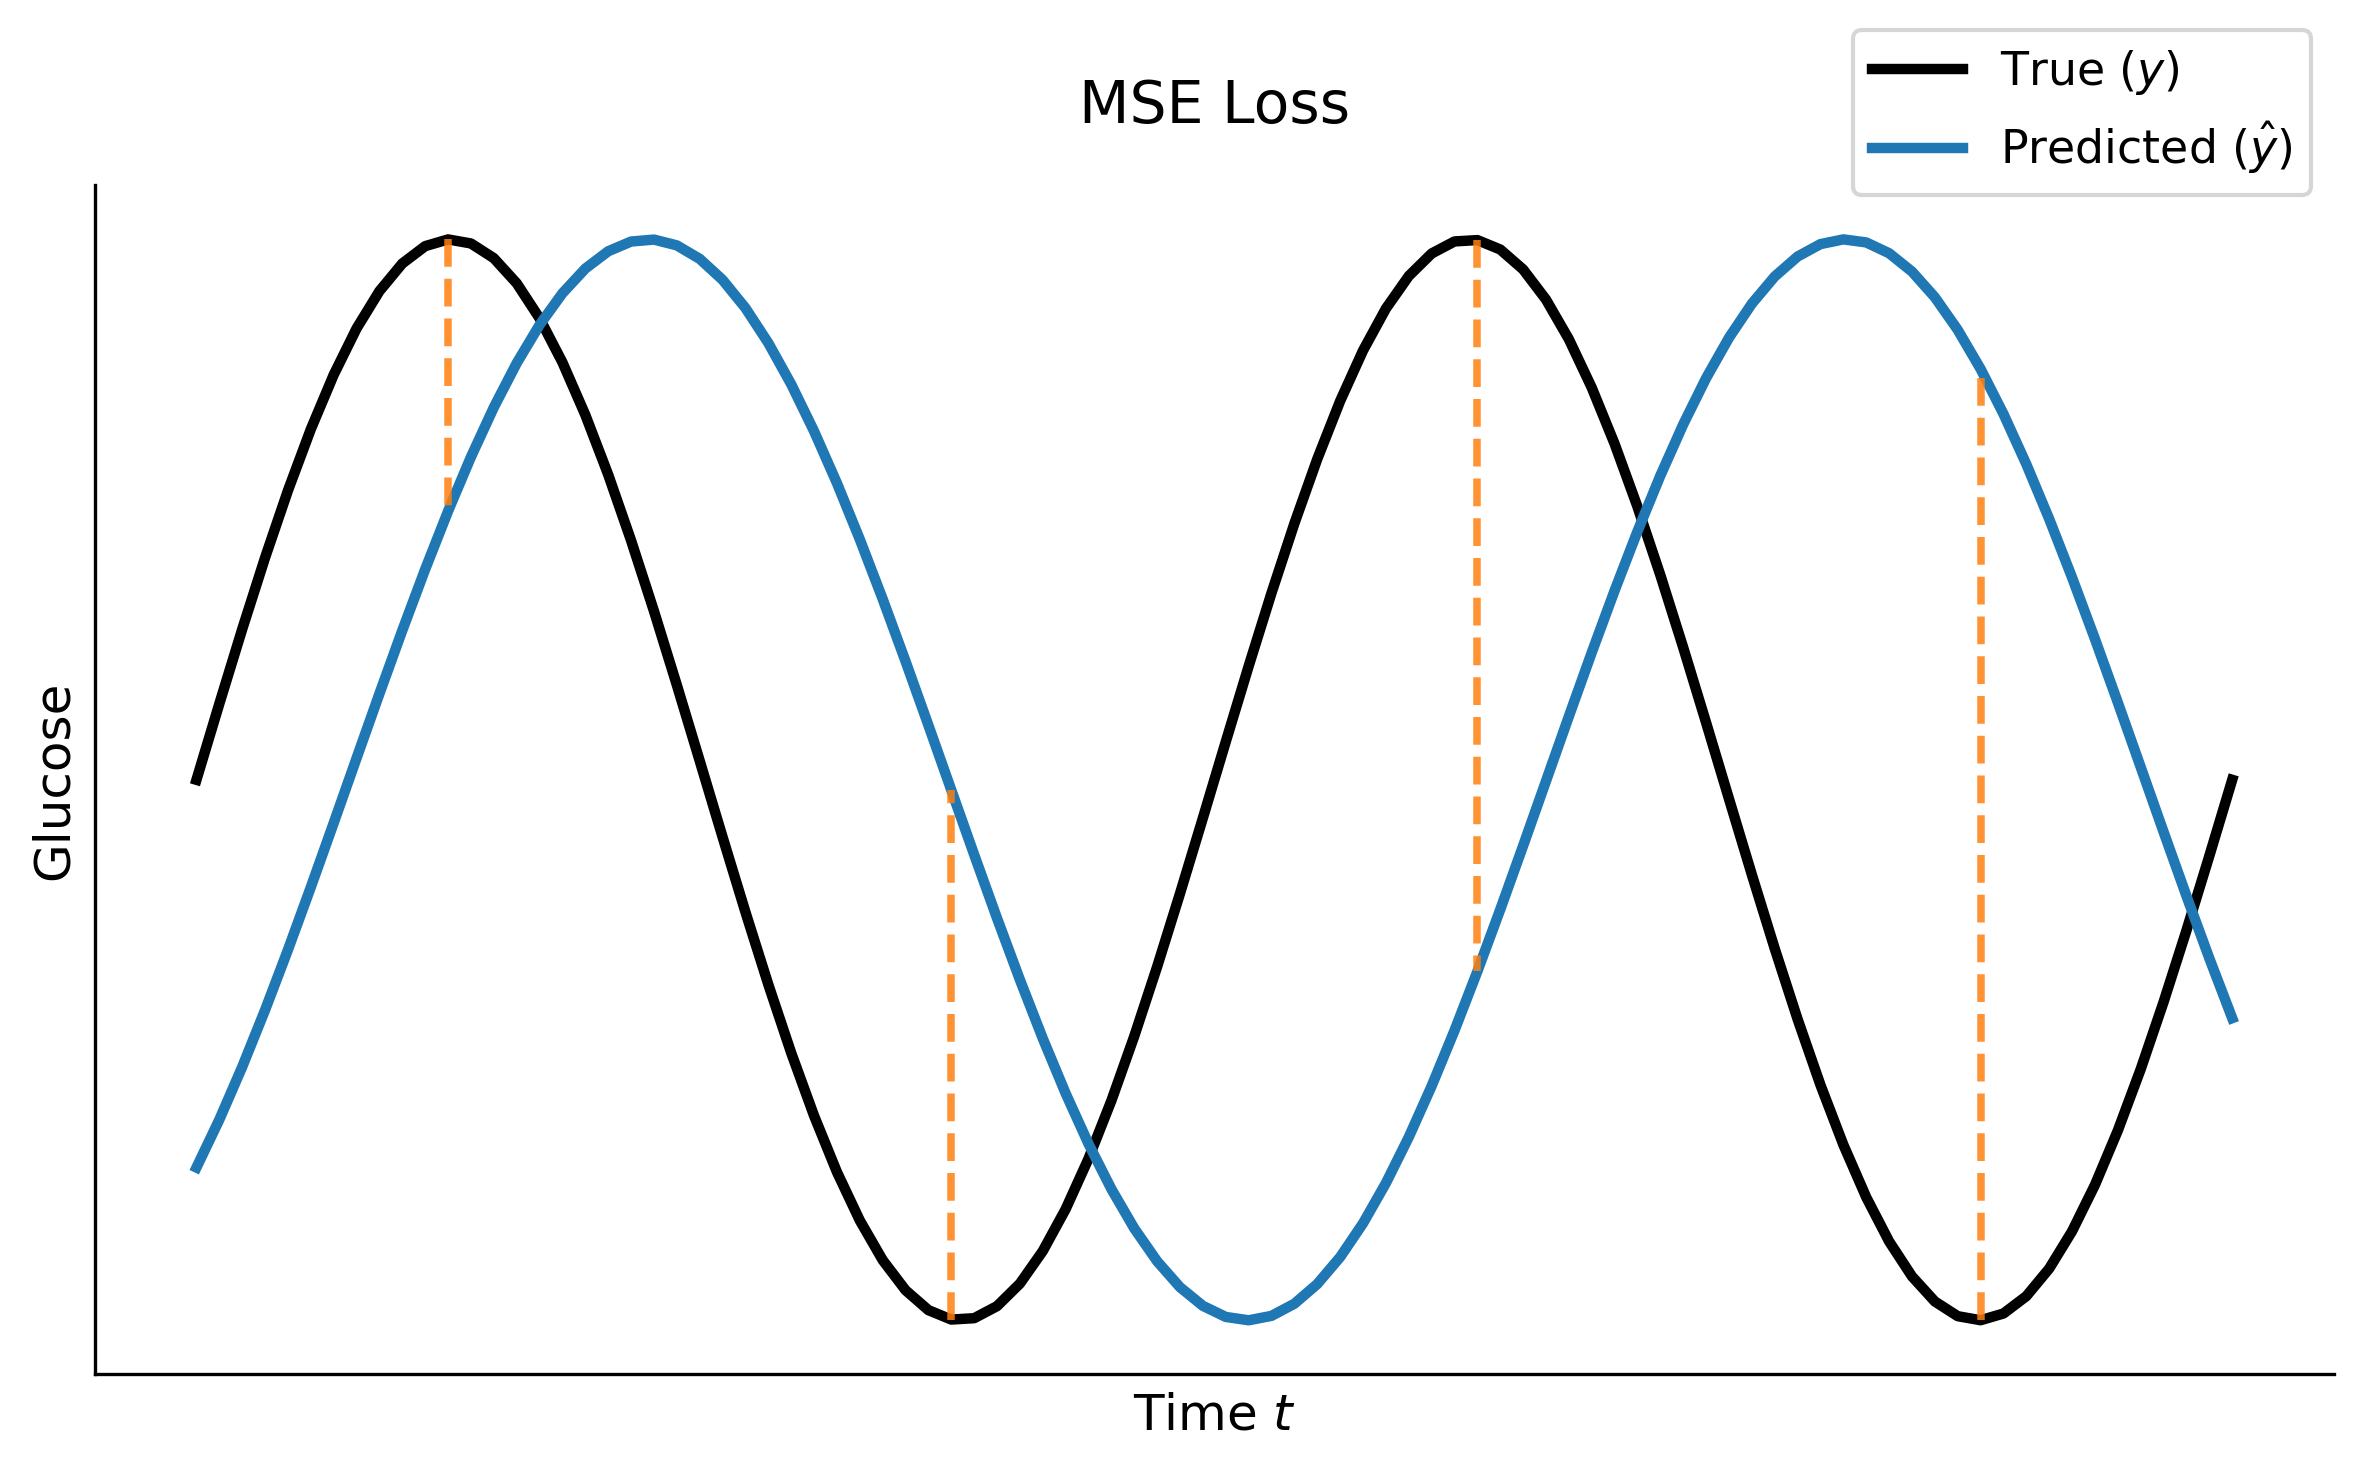
\includegraphics[width=0.75\textwidth]{loss_mse.png}
    \caption{Visual representation of the Mean Squared Error (MSE). The strict point-wise alignment heavily penalizes structurally correct predictions that are temporally delayed.}
    \label{fig:loss_mse}
\end{figure}

\subsection{Bounded Lag Loss} \label{sec:bg:losses:bl}
\begin{planned}
    \item Description of the Bounded Lag loss, which accepts a prediction as correct if it falls within a fixed time window of the true value, removing the penalty for small timing offsets.
\end{planned}

\begin{figure}[htbp]
    \centering
    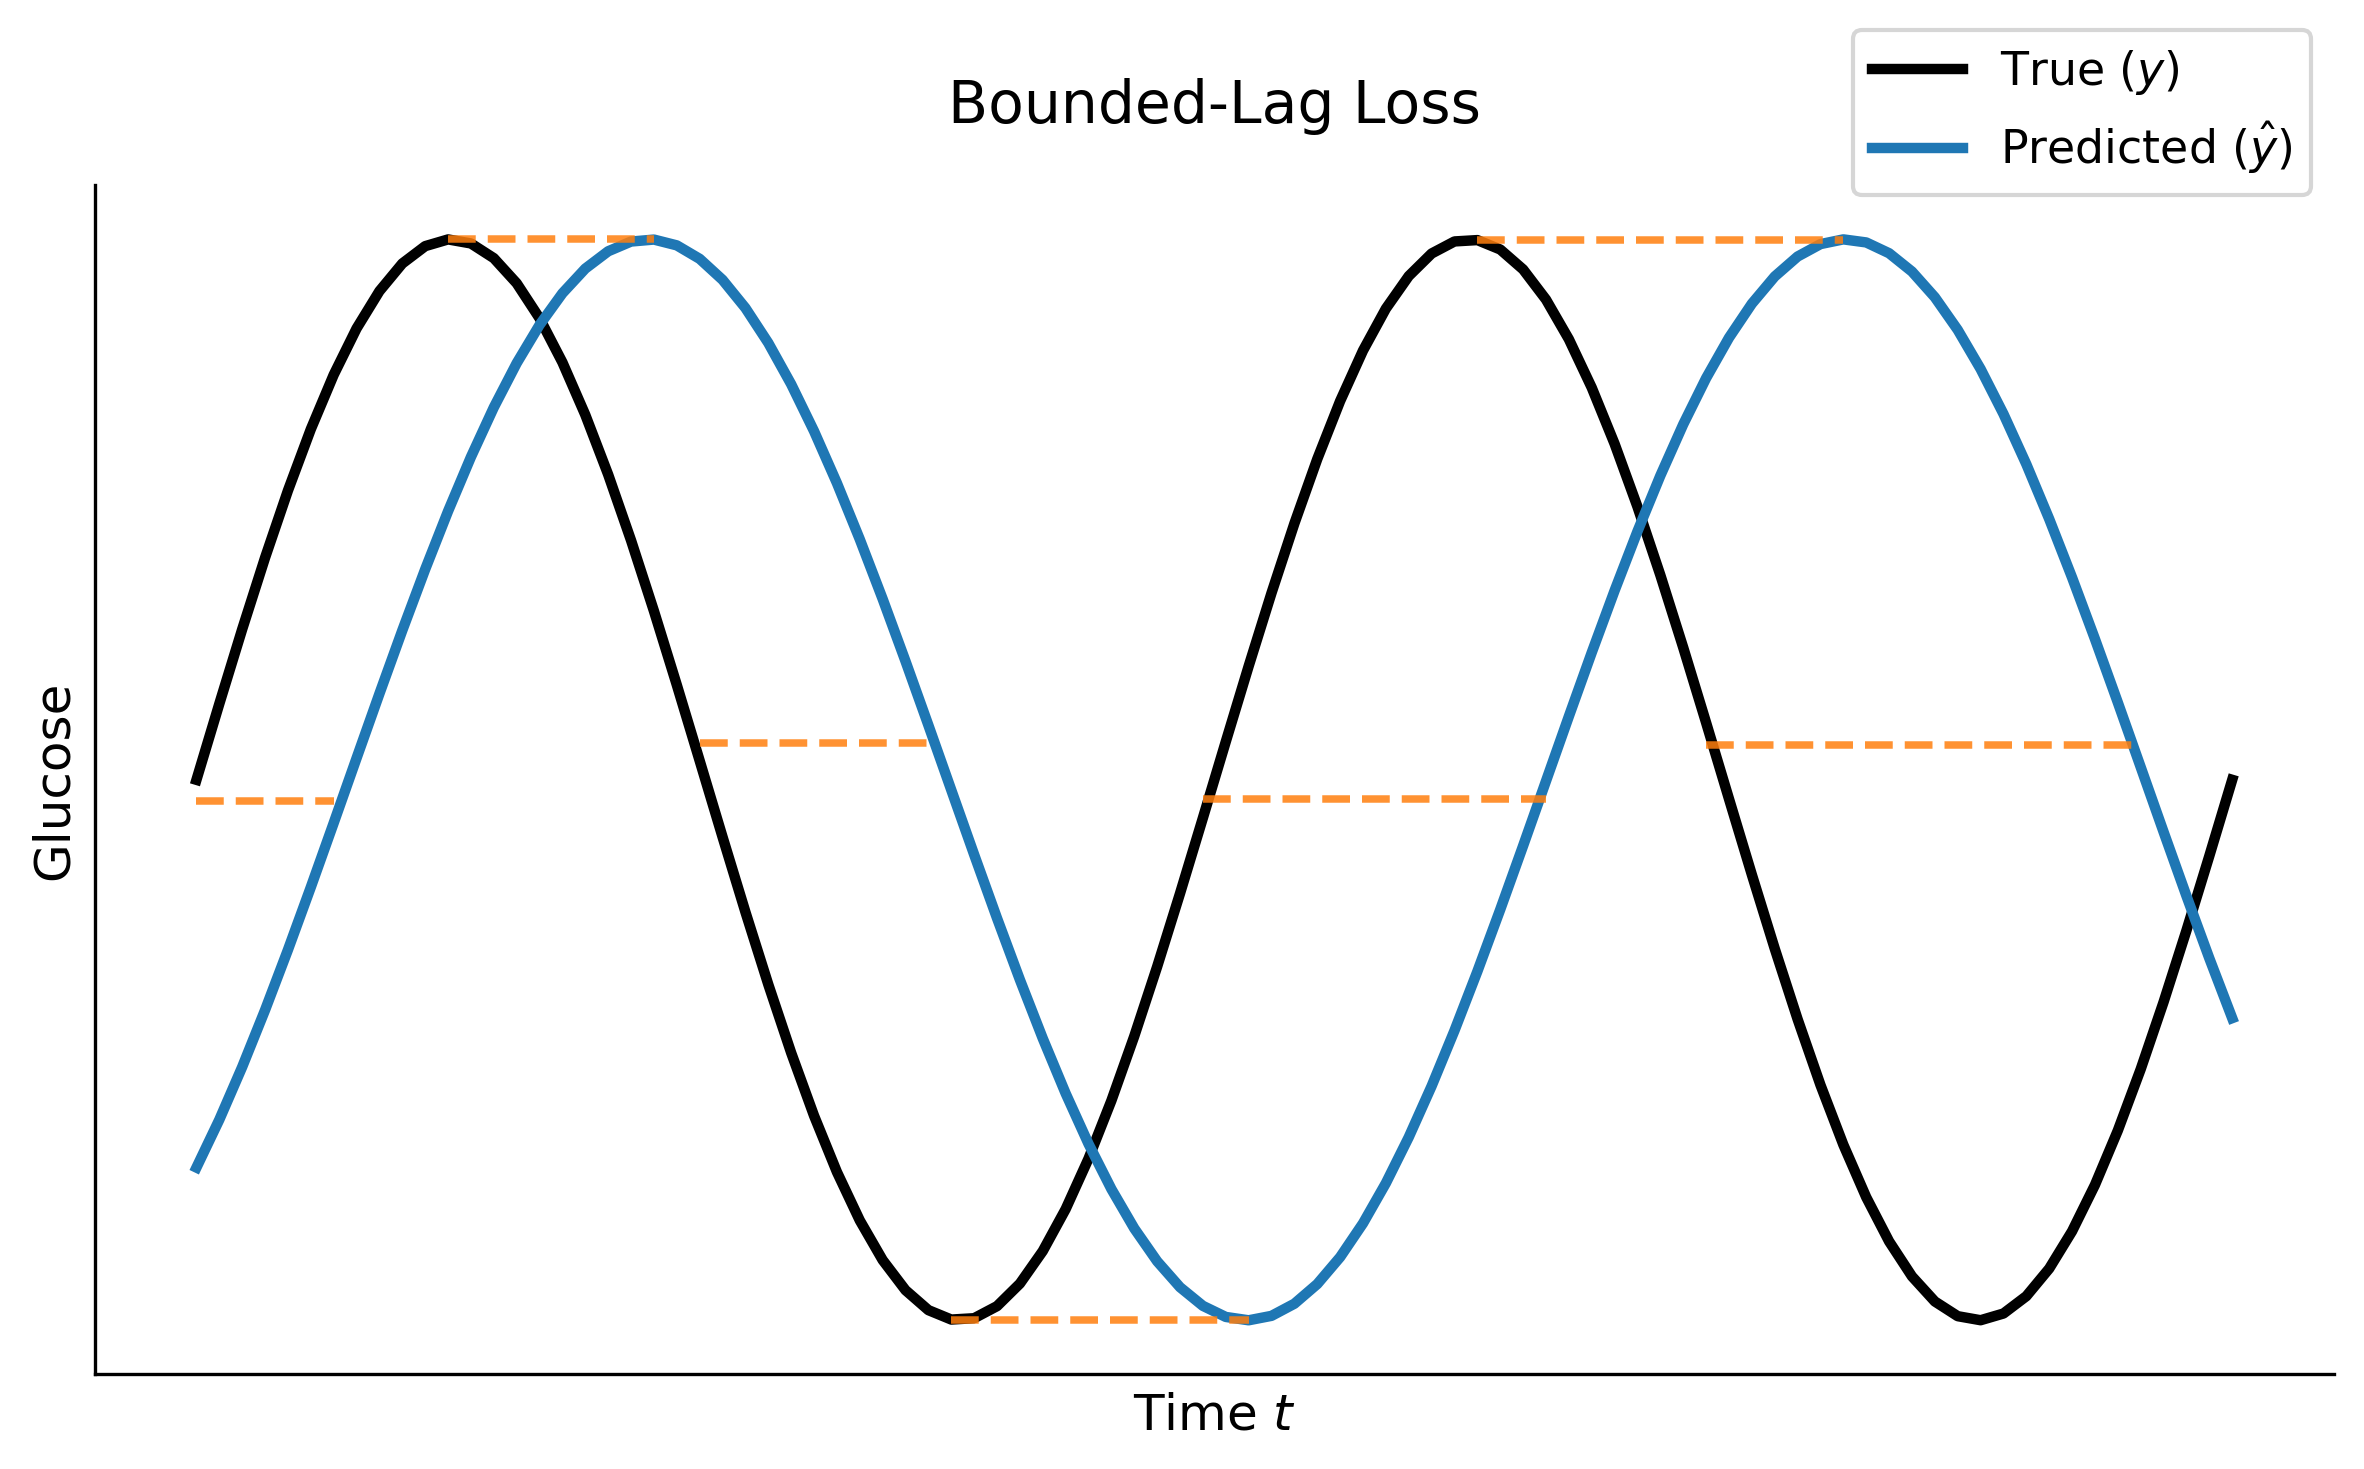
\includegraphics[width=0.75\textwidth]{loss_bounded_lag.png}
    \caption{Visual representation of the Bounded Lag Loss. Temporal shifts within a predefined local neighborhood are tolerated without penalty.}
    \label{fig:loss_bl}
\end{figure}

\subsection{Soft DTW: Differentiable Dynamic Time Warping} \label{sec:bg:losses:sdtw}
\begin{planned}
    \item Description of Soft DTW, which aligns two sequences by warping the time axis to match their shapes, allowing one-to-many correspondences between time steps.
    \item Trade-off: focusing on shape matching reduces the penalty for timing errors but can increase overall amplitude error.
\end{planned}

\begin{figure}[htbp]
    \centering
    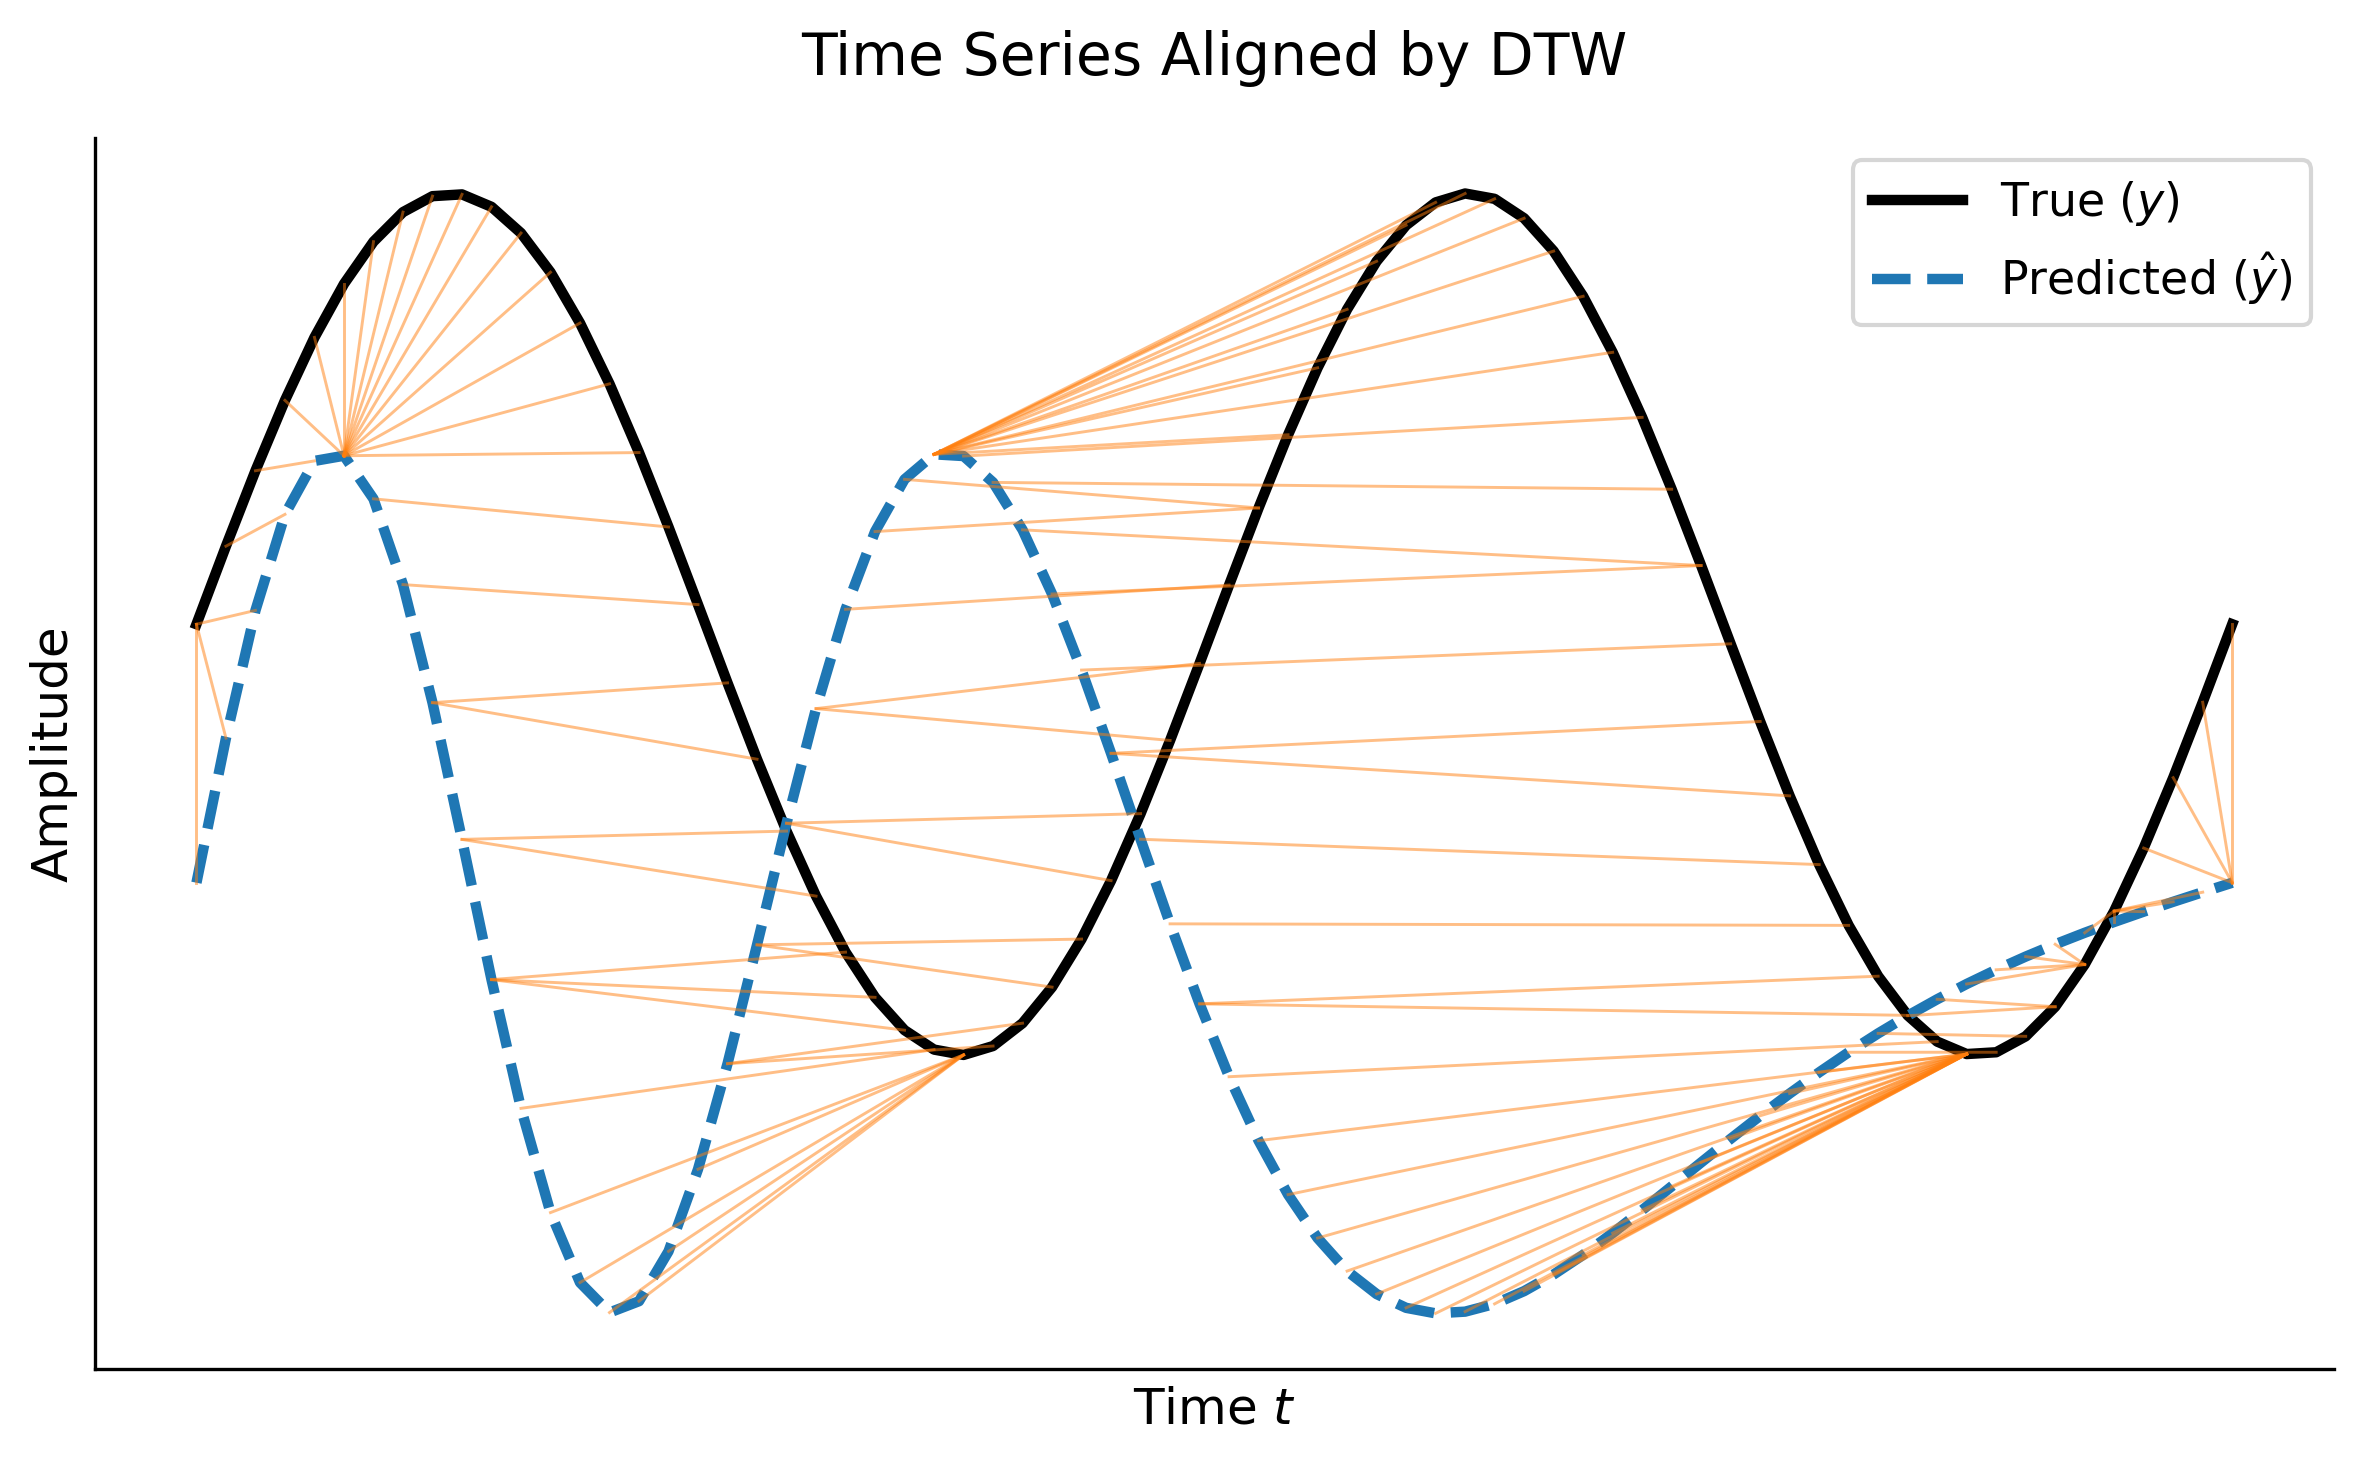
\includegraphics[width=0.75\textwidth]{loss_dtw_alignment.png}
    \caption{Visual representation of the Soft DTW Loss. The algorithm dynamically warps the time axis to match structural shapes using one-to-many alignments.}
    \label{fig:loss_dtw}
\end{figure}

% ================================================================
\section{Evaluation Metrics} \label{sec:bg:metrics}
% ================================================================
\begin{planned}
    \item Mathematical definitions of RMSE and MAE.
    \item Definition of the \texttt{lag\_rmse} diagnostic metric to quantitatively isolate temporal delay components.
    \item Derivation of precision, recall, and harmonic F1/F2 score metrics adapted to the evaluation of highly skewed event detection tasks.
\end{planned}

\begin{figure}[htbp]
    \centering
    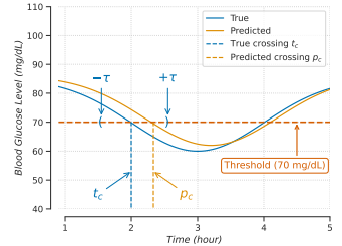
\includegraphics[width=0.7\textwidth]{tau_tolerance.png}
    \caption{Illustration of the event-detection tolerance window $\tau$. The true threshold crossing $t_c$ and the predicted crossing $p_c$ are considered a matched detection if $|t_c - p_c| \leq \tau$. The shaded $\pm\tau$ band around $t_c$ defines the acceptance region; predictions falling outside this window are counted as false positives or misses.}
    \label{fig:bg:tau_tolerance}
\end{figure}

\begin{figure}[htbp]
    \centering
    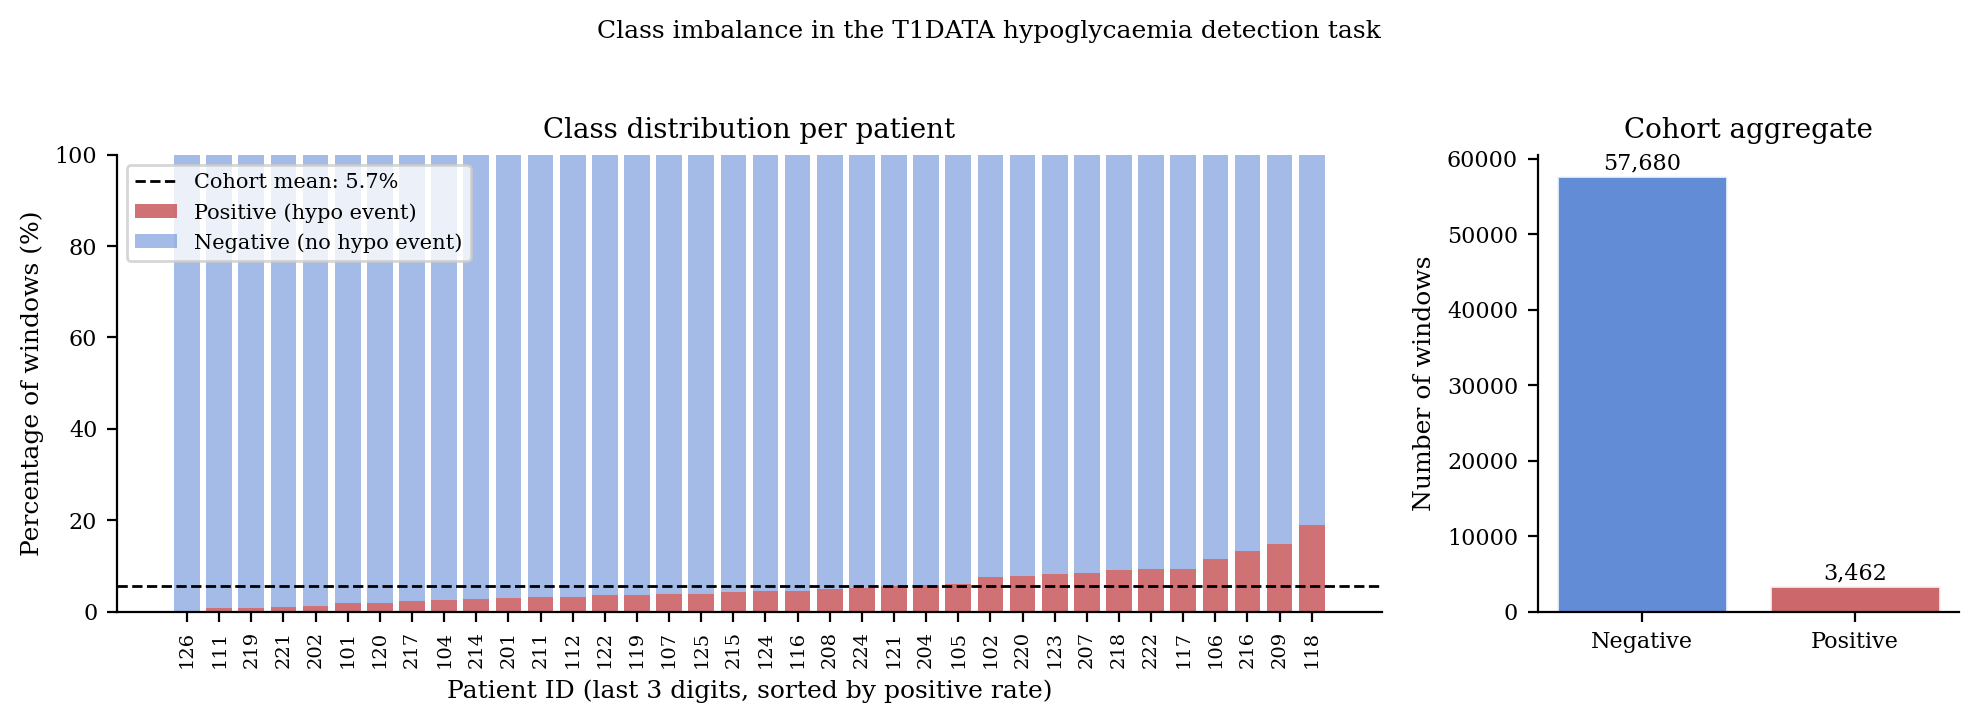
\includegraphics[width=\textwidth]{class_imbalance.png}
    \caption{Class distribution of the hypoglycaemia detection task across the 36-patient T1DATA cohort. Each window is labelled positive if glucose falls below 70~mg/dL within the next 60~minutes. Positive windows account for only 5.7\% of all labelled windows at cohort level (3{,}462 positive vs.\ 57{,}680 negative), with substantial variation across patients. This severe imbalance motivates the use of the F2 metric and inverse-frequency weighting in the binary cross-entropy loss for direct classifiers.}
    \label{fig:bg:class_imbalance}
\end{figure}

% ================================================================
\section{Related Work} \label{sec:bg:relwork}
% ================================================================
\begin{planned}
    \item Review of dominant recurrent and transformer-based neural structures applied within modern long-horizon metabolic time series prediction.
    \item Comparison of prior approaches, positioning this thesis explicitly within the gap of separating shape error from temporal misalignment.
\end{planned}
